\documentclass[a4paper, 10pt]{article}
%\usepackage{fontspec}
%\setmainfont{Lato}
\usepackage{pgf}
\usepackage{eurosym}
\usepackage{graphicx}
\usepackage{wasysym}
\usepackage{hyperref}
\usepackage{listings}
\usepackage{pxfonts}
\usepackage{verbatim}
\usepackage{color}
\usepackage{xcolor}
\usepackage{wrapfig}
\usepackage{enumitem}
\usepackage{booktabs}
\usepackage{gensymb}
\usepackage{tabularx}
\usepackage{currfile}

\hypersetup{
    bookmarks=true,         % show bookmarks bar?
    unicode=true,          % non-Latin characters in Acrobat’s bookmarks
    pdftoolbar=true,        % show Acrobat’s toolbar?
    pdfmenubar=true,        % show Acrobat’s menu?
    pdffitwindow=true,     % window fit to page when opened
    pdftitle={Assessments},    % title
    pdfauthor={Paul Vesey},     % author
    pdfsubject={Advanced Graphics Assignment },   % subject of the document
    pdfcreator={},   % creator of the document
    pdfproducer={xelatex}, % producer of the document
    pdfkeywords={'Graphics' }, % list of keywords
    pdfnewwindow=true,      % links in new PDF window
    colorlinks=true,       % false: boxed links; true: colored links
    linkcolor=violet,          % color of internal links (change box color with linkbordercolor)
    citecolor=magenta,        % color of links to bibliography
    filecolor=red,      % color of file links
    urlcolor=blue           % color of external links
}

\setlength\parindent{0pt}
\begin{document}

\lstset{language=HTML,
				basicstyle=\small,
				breaklines=true,
        numbers=left,
        numberstyle=\tiny,
        showstringspaces=false,
        aboveskip=-20pt,
        frame=leftline
        }
				
\begin{table}%
	\begin{minipage}{0.4\textwidth}%
			
\includegraphics[width=1\textwidth]{./img/LITlogo.jpg}
	\end{minipage}
	\qquad
	\centering
	\parbox{0.4\textwidth}{
		\begin{large}			
			\begin{tabular}{| r | l |} \hline
				Subject: & \textbf{Advanced Graphics}\\
								 & \textbf{\& Visualisation}\\
				Course: & \textbf{Interior Design Y3}\\
				Session: & \textbf{Autumn 2020}\\
				Lecturer: & \textbf{Paul Vesey \footnotesize{BEng, MIE, HDip}}\\
				Filename: & \footnotesize{\currfilename}\\
				\hline
			\end{tabular}
		\end{large}			
	}
\end{table}
\vspace{0.25cm}	
	
\begin{flushleft}
\Large\textbf{Practical 2 - Practical Modeling }\\
\end{flushleft}

In this practical you are going to develop your building modeling skills using two of the main model creation processes, namely poly-modeling from scratch, and modeling from an existing Autocad drawing\\


\textbf{Poly-model from Scratch}\\
Key Dimensions for the poly-model are:
\begin{itemize}
	\item Length: 5000mm
	\item Width: 4000mm
	\item Height: 2300mm
	\item Sill height 900mm
	\item Header height (doors \& windows) 2040mm
\end{itemize}

Key Functions are:
\begin{itemize}
	\item Extrude
	\item Slice
	\item Bridge
	\item Connect
\end{itemize}

\begin{figure}[ht]
	\centering
		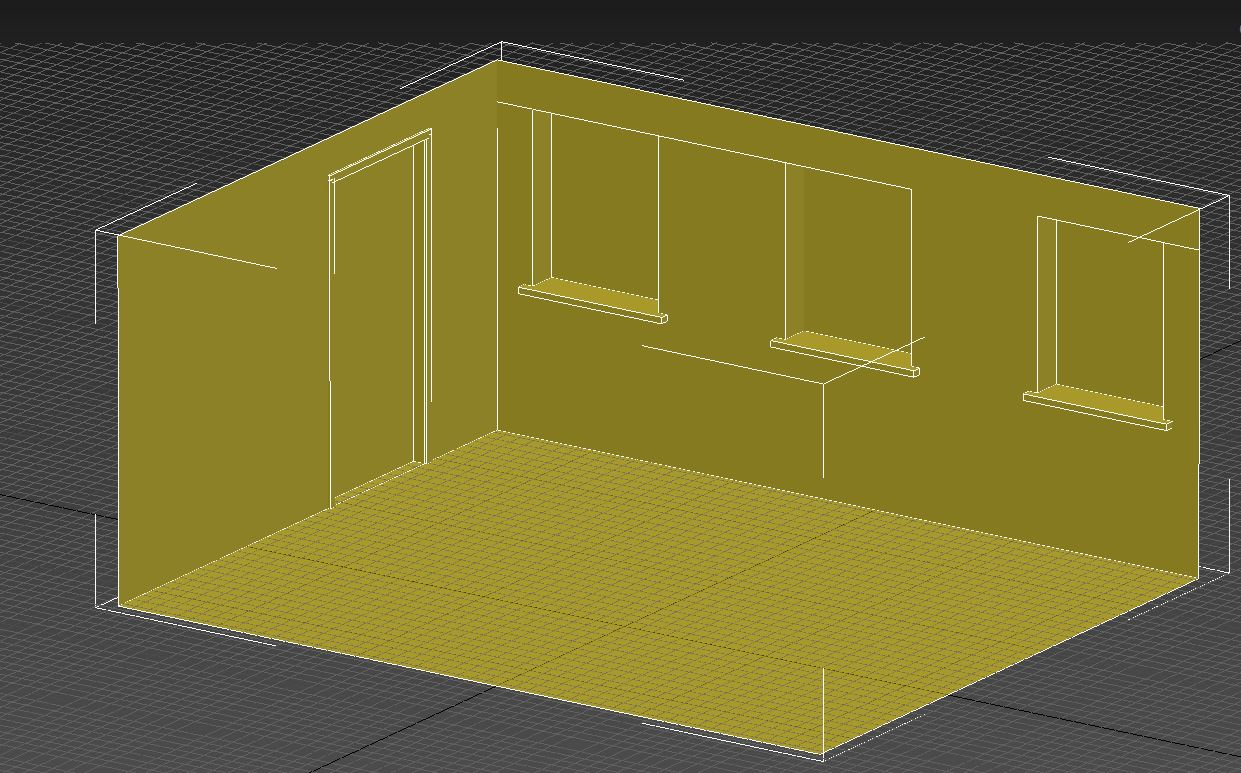
\includegraphics[width=10cm]{./img/PolyModel.jpg}
		\caption{Basic Polygon Model}
	\label{fig:PM}
\end{figure}


\newpage
\vspace{1cm}
\begin{figure}[ht]
	\centering
		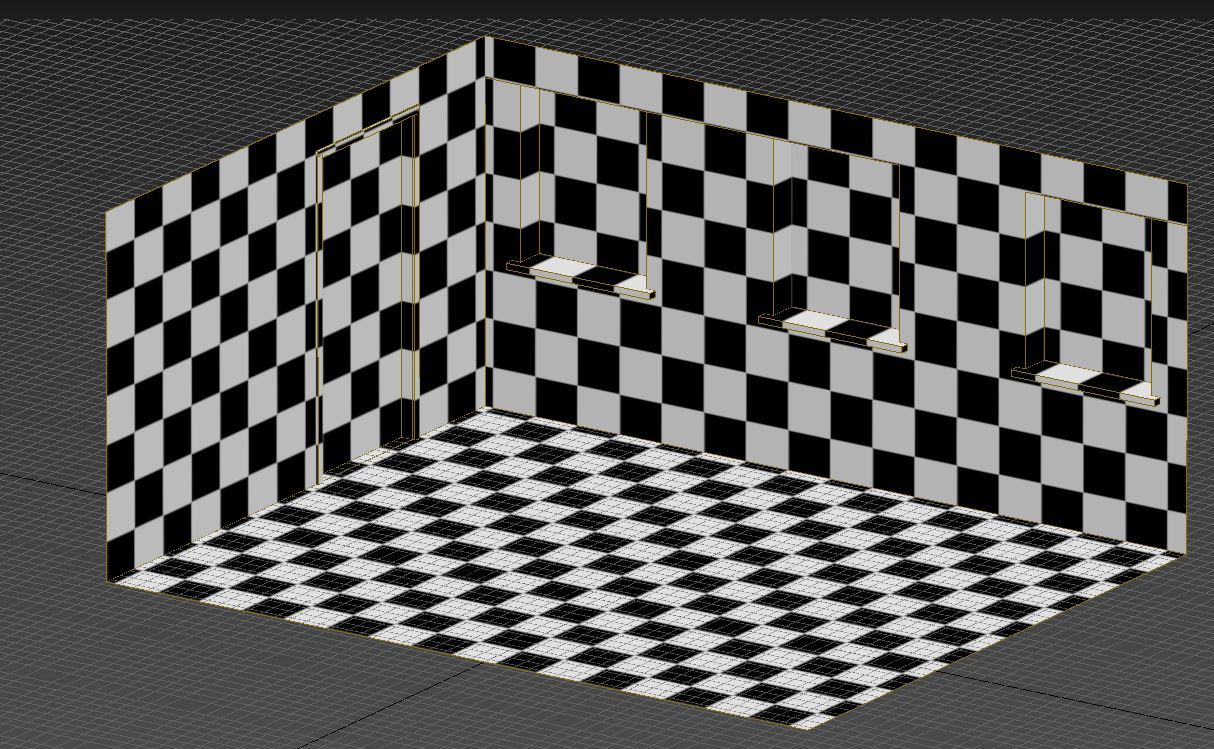
\includegraphics[width=10cm]{./img/PolyModelCheck.jpg}
		\caption{UVW Model Check}
	\label{fig:PMC}
\end{figure}


\vspace{1cm}
\begin{figure}[ht]
	\centering
		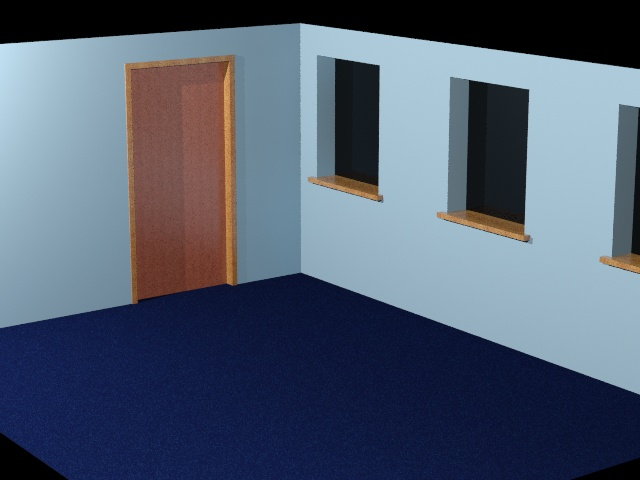
\includegraphics[width=10cm]{./img/SimpleRender.jpg}
		\caption{Simple Render}
	\label{fig:Simplerender}
\end{figure}

\newpage

\textbf{Import from Autocad}\\
The commands for the Autocad drawing are the same as before; however in this case you will first have to import the AutoCAD drawing from the asset pack

\begin{figure}[hb]
	\centering
		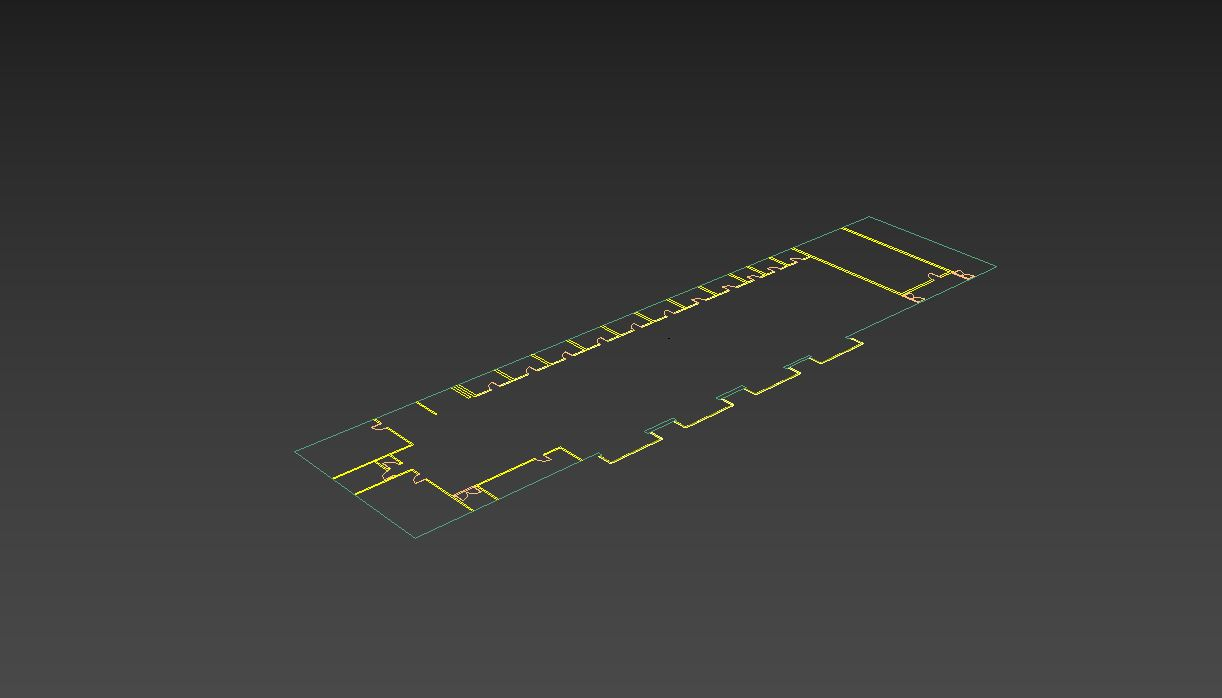
\includegraphics[width=10cm]{./img/DwgImported.jpg}
		\caption{Imported Autocad Drawing}
	\label{fig:DwgImported}
\end{figure}


\begin{figure}[hb]
	\centering
		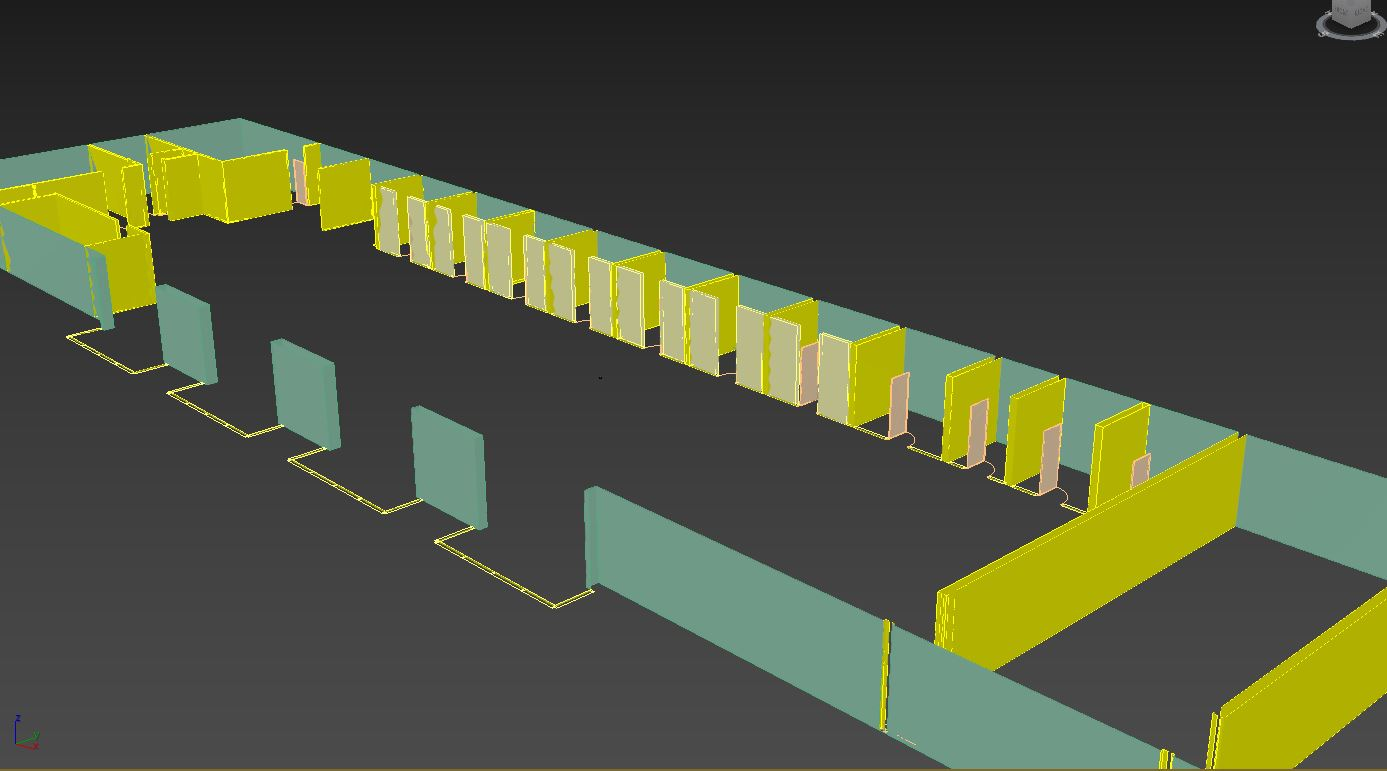
\includegraphics[width=10cm]{./img/DwgWIP.jpg}
		\caption{3D Model in progress (WIP)}
	\label{fig:DwgWIP}
\end{figure}





The asset pack for this assignment can be downloaded from \href{https://goo.gl/AGqD5a}{https://goo.gl/AGqD5a}\\

You are not required to submit your completed models; they will not form part of your final grade in this subject.\\

\end{document}